\documentclass[12pt, twoside]{article}
\usepackage[letterpaper, margin=1in, headsep=0.2in]{geometry}
\setlength{\headheight}{0.6in}
%\usepackage[english]{babel}
\usepackage[utf8]{inputenc}
\usepackage{microtype}
\usepackage{amsmath}
\usepackage{amssymb}
%\usepackage{amsfonts}
\usepackage{siunitx} %units in math. eg 20\milli\meter
\usepackage{yhmath} % for arcs, overparenth command
\usepackage{tikz} %graphics
\usetikzlibrary{quotes, angles}
\usepackage{graphicx} %consider setting \graphicspath{{images/}}
\usepackage{parskip} %no paragraph indent
\usepackage{enumitem}
\usepackage{multicol}
\usepackage{venndiagram}

\usepackage{fancyhdr}
\pagestyle{fancy}
\fancyhf{}
\renewcommand{\headrulewidth}{0pt} % disable the underline of the header
\raggedbottom
\hfuzz=2mm %suppresses overfull box warnings

\usepackage{hyperref}

\fancyhead[LE]{\thepage}
\fancyhead[RO]{\thepage \\ Name: \hspace{4cm} \,\\}
\fancyhead[LO]{BECA / Dr. Huson / Geometry\\*  Unit 8: Year-to-date Regents review\\* 3 March 2023}

\begin{document}

\subsubsection*{8.6 Quiz: Triangle angles, transversals, segments, solids}
\begin{enumerate}
\item Find the volume of a rectangular prism with length 5 cm, width 10 cm, and height 8 cm. \vspace{2cm}

\item Find the volume of a pyramid ($V=\frac{1}{3}Bh$) having a height of 13 inches and with a square base having side lengths of 6 inches. Express your result to the \emph{nearest cubic inch}. \vspace{3cm}


\item Find the volume of a sphere with a radius of 3 inches, to the \emph{nearest whole cubic inch}. (The formula for the volume of a \emph{sphere} is $V=\frac{4}{3}\pi r^3$) \vspace{4cm}

\item A child's tent can be modeled as a pyramid with a square base whose sides measure 60 inches and whose height measures 84 inches. What is the volume of the tent, to the \emph{nearest cubic foot}?

\newpage
\item Randy's basketball is in the shape of a sphere with a maximum circumference of 29.5 inches. Determine and state the volume of the basketball, to the \emph{nearest cubic inch}. \vspace{4cm}

\item The base of a pyramid is a rectangle with a width of 4.6 cm and a
length of 9 cm. What is the height, in centimeters, of the pyramid if
its volume is 82.8 cm$^3$? \vspace{4cm}

\item As shown in the diagram below, the radius of a cone is 2.5 cm and its slant height is 6.5 cm.
  \begin{center}
    \begin{tikzpicture}[scale=0.9]
    \draw [thick] (0,0)--(2.5,0)--(0,6)--cycle;
    \draw (0,0)++(0.4,0)--++(0,0.4)--+(-0.4,0);
    \draw [thick] (0,6)--(-2.5,0);
    \node at (1,0)[below]{$2.5$};
    \node at (1.7,3.2){$6.5$};
    \draw [dashed] (0,0) ellipse [x radius=2.5,y radius=0.6];
    \clip (-3,-2) rectangle (3,0);
    \draw [thick] (0,0) ellipse [x radius=2.5,y radius=0.6];
  \end{tikzpicture}
  \end{center}
How many cubic centimeters are in the volume of the cone? Express your answer in terms of $\pi$. \vspace{3cm}

\newpage
\item Lou has a solid clay brick in the shape of a rectangular prism with a length of 8 inches, a width of 3.5 inches, and a height of 2.25 inches. If the clay weighs 1.055 oz/in$^3$, how much does Lou's brick weigh, to the nearest ounce? \vspace{4cm}

\item A rectangular tabletop will be made of maple wood that weighs 43 pounds per cubic foot. The tabletop will have a length of eight feet, a width of three feet, and a thickness of one inch. Determine and state the weight of the tabletop, in pounds. \vspace{4cm}

\item A cone has a volume of $108\pi$ and a base diameter of 12. What is the
height of the cone? \vspace{4cm}

\subsubsection*{3-D rotation}
\item If a right triangle is continuously rotated around one of its legs (not the hypotenuse), what is the three-dimensional figure formed?
  \begin{multicols}{2}
  \begin{enumerate}
    \item cone
    \item sphere
    \item cylinder
    \item rectangular prism
  \end{enumerate}
\end{multicols}


\end{enumerate}
\end{document}